\documentclass[journal]{vgtc}                % final (journal style)
%\documentclass[review,journal]{vgtc}         % review (journal style)
%\documentclass[widereview]{vgtc}             % wide-spaced review
%\documentclass[preprint,journal]{vgtc}       % preprint (journal style)

%% Uncomment one of the lines above depending on where your paper is
%% in the conference process. ``review'' and ``widereview'' are for review
%% submission, ``preprint'' is for pre-publication, and the final version
%% doesn't use a specific qualifier.

%% Please use one of the ``review'' options in combination with the
%% assigned online id (see below) ONLY if your paper uses a double blind
%% review process. Some conferences, like IEEE Vis and InfoVis, have NOT
%% in the past.

%% Please use the ``preprint''  option when producing a preprint version
%% for sharing your article on an open access repository

%% Please note that the use of figures other than the optional teaser is not permitted on the first page
%% of the journal version.  Figures should begin on the second page and be
%% in CMYK or Grey scale format, otherwise, colour shifting may occur
%% during the printing process.  Papers submitted with figures other than the optional teaser on the
%% first page will be refused. Also, the teaser figure should only have the
%% width of the abstract as the template enforces it.

%% These few lines make a distinction between latex and pdflatex calls and they
%% bring in essential packages for graphics and font handling.
%% Note that due to the \DeclareGraphicsExtensions{} call it is no longer necessary
%% to provide the the path and extension of a graphics file:
%% 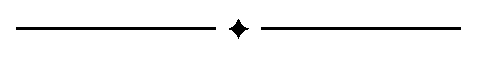
\includegraphics{diamondrule} is completely sufficient.
%%
\ifpdf%                                % if we use pdflatex
  \pdfoutput=1\relax                   % create PDFs from pdfLaTeX
  \pdfcompresslevel=9                  % PDF Compression
  \pdfoptionpdfminorversion=7          % create PDF 1.7
  \ExecuteOptions{pdftex}
  \usepackage{graphicx}                % allow us to embed graphics files
  \DeclareGraphicsExtensions{.pdf,.png,.jpg,.jpeg} % for pdflatex we expect .pdf, .png, or .jpg files
\else%                                 % else we use pure latex
  \ExecuteOptions{dvips}
  \usepackage{graphicx}                % allow us to embed graphics files
  \DeclareGraphicsExtensions{.eps}     % for pure latex we expect eps files
\fi%

%% it is recomended to use ``\autoref{sec:bla}'' instead of ``Fig.~\ref{sec:bla}''
\graphicspath{{figures/}{pictures/}{images/}{./}} % where to search for the images

\usepackage{microtype}                 % use micro-typography (slightly more compact, better to read)
\PassOptionsToPackage{warn}{textcomp}  % to address font issues with \textrightarrow
\usepackage{textcomp}                  % use better special symbols
\usepackage{mathptmx}                  % use matching math font
\usepackage{times}                     % we use Times as the main font
\renewcommand*\ttdefault{txtt}         % a nicer typewriter font
\usepackage{cite}                      % needed to automatically sort the references
%% We encourage the use of mathptmx for consistent usage of times font
%% throughout the proceedings. However, if you encounter conflicts
%% with other math-related packages, you may want to disable it.
\usepackage{amsmath,amsfonts,amssymb,pxfonts,eulervm,xspace}
\usepackage{mathrsfs} % math script fonts
\usepackage{tabulary}
\usepackage[utf8]{inputenc}
\usepackage{subfig} %ieee does not like subfigure
\usepackage{multicol}
\usepackage{tikz}
\usetikzlibrary{cd} % commutative diagrams
\newtheorem{prop}{Proposition} %math?
\usepackage[switch]{lineno}
\usepackage{minted}
\setminted[python]{fontsize=\scriptsize, 
                   linenos,
                   numbersep=8pt,
                   autogobble, 
                   frame=lines,
                   framesep=3mm} 
\usepackage{notation} % move this later


%% In preprint mode you may define your own headline. If not, the default IEEE copyright message will appear in preprint mode.
%\preprinttext{To appear in IEEE Transactions on Visualization and Computer Graphics.}

%% In preprint mode, this adds a link to the version of the paper on IEEEXplore
%% Uncomment this line when you produce a preprint version of the article 
%% after the article receives a DOI for the paper from IEEE
%\ieeedoi{xx.xxxx/TVCG.201x.xxxxxxx}

%% If you are submitting a paper to a conference for review with a double
%% blind reviewing process, please replace the value ``0'' below with your
%% OnlineID. Otherwise, you may safely leave it at ``0''.
\onlineid{0}

%% declare the category of your paper, only shown in review mode
\vgtccategory{Research}
%% please declare the paper type of your paper to help reviewers, only shown in review mode
%% choices:
%% * algorithm/technique
%% * application/design study
%% * evaluation
%% * system
%% * theory/model
\vgtcpapertype{Theory/Model}

%% Paper title.
\title{Topological Equivariant Artist Model}

%% This is how authors are specified in the journal style

%% indicate IEEE Member or Student Member in form indicated below
\author{Hannah Aizenman, Thomas Caswell, Michael Grossberg}
\authorfooter{
%% insert punctuation at end of each item
\item
 Hannah Aizenman and Michael Grossberg are with the department of Computer Science, City College of New York. E-mail: haizenman@ccny.cuny.edu, mgrossberg@ccny.cuny.edu.
\item
 Thomas Caswell is with National Synchrotron Light Source II, Brookhaven National Lab E-mail: tcaswell@bnl.gov.
}

%other entries to be set up for journal
\shortauthortitle{Aizenman \MakeLowercase{\textit{et al.}}: Topological Equivariant Artist Model}
%\shortauthortitle{Firstauthor \MakeLowercase{\textit{et al.}}: Paper Title}

%% Abstract section.
\abstract{This work presents a functional model of the structure-preserving maps from data to visual representation to guide the development of visualization libraries. Our model, which we call the  topological equivariant artist model (TEAM), provides a means to express the constraints of preserving the data continuity in the graphic and faithfully translating the properties of the data variables into visual variables. We formalize these transformations as actions on sections of topological fiber bundles, which are mathematical structures that allow us to encode continuity as a base space, variable properties as a fiber space, and data as binding maps, called sections, between the base and fiber spaces. This abstraction allows us to generalize to any type of data structure, rather than assuming, for example, that the data is a relational table, image, data cube, or network-graph. Moreover, we extend the fiber bundle abstraction to the graphic objects that the data is mapped to. By doing so, we can track the preservation of data continuity in terms of continuous maps from the base space of the data bundle to the base space of the graphic bundle. Equivariant maps on the fiber spaces preserve the structure of the variables; this structure can be represented in terms of monoid actions, which are a generalization of the mathematical structure of Stevens’ theory of measurement scales. We briefly sketch that these transformations have an algebraic structure which lets us build complex components for visualization from simple ones. We demonstrate the utility of this model through case studies of a scatter plot, line plot, and image. To demonstrate the feasibility of the model, we implement a prototype of a scatter and line plot in the context of the Matplotlib Python visualization library.  We propose that the functional architecture derived from a TEAM based design specification can provide a basis for a more consistent API and better modularity, extendability, scaling and support for concurrency} 

% end of abstract

%% Keywords that describe your work. Will show as 'Index Terms' in journal
%% please capitalize first letter and insert punctuation after last keyword
% http://ieeevis.org/year/2021/info/call-participation/paper-keywords
\keywords{Taxonomy, Models, Frameworks, Theory}

%% ACM Computing Classification System (CCS). 
%% See <http://www.acm.org/class/1998/> for details.
%% The ``\CCScat'' command takes four arguments.
%https://www.acm.org/publications/computing-classification-system/1998/top
\CCScatlist{ % not used in journal version
 \CCScat{I.3.6}{Computer Graphics}%
{Methodology and Techniques}{Graphics data structures and data types};}

%% A teaser figure can be included as follows
\teaser{
  \centering
  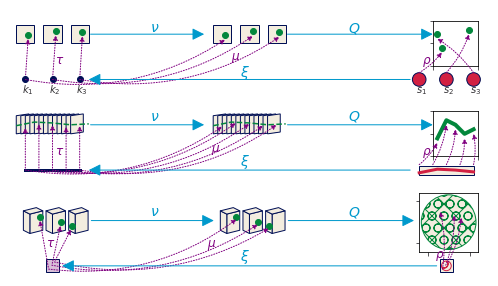
\includegraphics[width=\linewidth]{teaser.png}
  \caption{Visualizations consist of topologically equivariant maps. There is a set of monoid action equivariant maps from data components to visual components \vchannel\ that are then reduced via \vmark\ into a single graphic, and there is a deformation retraction \vindex\ from graphic continuity to data continuity.}
  \label{fig:teaser}
}


%% Uncomment below to disable the manuscript note
%\renewcommand{\manuscriptnotetxt}{}

%% Copyright space is enabled by default as required by guidelines.
%% It is disabled by the 'review' option or via the following command:
% \nocopyrightspace


\vgtcinsertpkg

%%%%%%%%%%%%%%%%%%%%%%%%%%%%%%%%%%%%%%%%%%%%%%%%%%%%%%%%%%%%%%%%
%%%%%%%%%%%%%%%%%%%%%% START OF THE PAPER %%%%%%%%%%%%%%%%%%%%%%
%%%%%%%%%%%%%%%%%%%%%%%%%%%%%%%%%%%%%%%%%%%%%%%%%%%%%%%%%%%%%%%%%

\begin{document}
\linenumbers %linenumbers for comments [make sure to remove later]
%% The ``\maketitle'' command must be the first command after the
%% ``\begin{document}'' command. It prepares and prints the title block.

%% the only exception to this rule is the \firstsection command
\firstsection{Introduction}
\maketitle
%% this is still a mess, come back to it

General purpose visualization libraries are often tasked with supporting many domains, leading the libraries to grow organically in ways that can lead to incoherent interfaces and brittle components. To adapt to modern library development needs, this paper presents a functional model of the how components provided by lower level libraries\cite{wongsuphasawatNavigatingWideWorld2021} can be guaranteed to be structure preserving maps from data to graphic. We target this level of library architecture because our aim is the libraries developers use to build automated and user facing tools, not those tools themselves; we are agnostic to what makes for a good visualization so long as the structure preserving constraints are satisfied. 
\begin{figure}[H]
  \centering 
  \subfloat[\label{fig:intro:continuity}]{%
    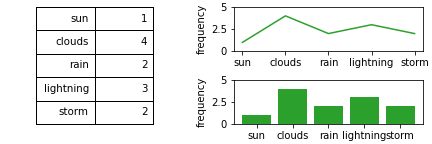
\includegraphics[width=1\columnwidth]{continuity.png}}\\
  \subfloat[\label{fig:intro:equivariance}]{%
    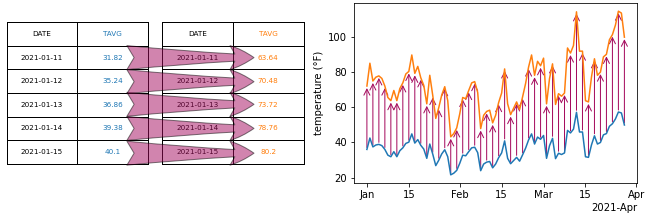
\includegraphics[width=1\columnwidth]{equivariance.png}}
\caption{In \autoref{fig:intro:continuity}, the line plot does not preserve \textit{continuity} because it implies that the discrete records are connected to each other, while the bar plot is \textit{continuity} preserving because it visually represents the records as independent data points. In \autoref{fig:intro:equivariance}, the data in blue is scaled by a factor of two, yielding the data in orange. To preserve \textit{equivariance}, the blue line plot representation of the unscaled data is also scaled by a factor of two, yielding the orange line plot that is equivalent to the scaled data.}
\label{fig:intro:structure}
\end{figure}
The structure that components of a visualization library must preserve is \textit{continuity} and \textit{equivariance}, as illustrated in \autoref{fig:intro:structure}. \textit{Continuity} is the way in which the records in the dataset are connected to each other. In \autoref{fig:intro:continuity}, the line plot does not preserve continuity because the line connecting the discrete categories implies that the frequency of weather events is sampled from a continuous interval and the categories are points on that interval. \textit{Equivariance} means that if any action is applied to the data or the visual, for example a rotation, permutation, translation, or rescaling, an equivalent action is applied on the other side. In \autoref{fig:intro:equivariance}, the data and visual representation are scaled by equivalent factors of two, resulting in the change illustrated in the shift from orange to blue.  

Motivated by the challenge of re-architecturing the Python visualization library Matplotlib, we developed a functional model of library architecture, which we call the Topological Equivariant Artist Model (TEAM), to specify the constraints components must satisfy to be equivariant continuity preserving mappings from data to visual representation. A functional architecture derived from our model would gain a generalized data abstraction and well specified reusable components with minimal side effects\cite{loudenProgrammingLanguagesPrinciples2010}, in turn yielding improvements in maintainability, extendability, scaling, and support for concurrency. The contribution of this work is 
\begin{enumerate}
  \item formalization of the topology preserving relationship between data and graphic via continuous maps \autoref{sec:math:graphic:base}
  \item formalization of property preservation from data component to visual representation as monoid action equivariant maps \autoref{sec:math:artist}
  \item functional oriented visualization architecture built on the mathematical model to demonstrate the utility of the model \autoref{sec:math:artist:q}
  \item prototype of the architecture built on Matplotlib's infrastructure to demonstrate the feasibility of the model. \autoref{sec:code}
\end{enumerate}

\section{Related Work}
The notion that visualization is equivariant continuity preserving maps from data to visual representation is neither a new formalism nor a new implementation goal, but this work bridges the formalism and implementation in a functional manner at a building building blocks library level. When introducing the retinal variables, Bertin informally introduces the notion that continuity is preserved in the mark and  defines equivariance constraints (selective, associative, ordered, quantitative)\cite{bertinSemiologyGraphicsDiagrams2011a}. In the \textit{A Presentation Tool}(APT) model, Mackinlay embeds the continuity constraint in the choice of visualization type and generalizes the equivariance constraint to preserving a binary operator from one domain to another. The algebraic model of visualization proposed by Kindlmann and Scheidegger restrict equivarance to group actions, but explicitly define composable symmetric mappings from data space to representation space to graphic space. Our model targets monoid actions as they are more restrictive than all binary operations but more general than groups, and explicitly formalizes the way in which continuity is preserved as topologically maps. APT and the algebraic model are also targeted at visual designs and tools that automatically generate those designs, while our model targets the tools that build those tools. 

Current visualization tools tend to either be architectured around a core data structure\cite{HeerSoftware2006} or explicitly implement the visual algorithm in terms of the data continuity the algorithm expects \cite{toryRethinkingVisualizationHighlevel2004}.  For example, the relational database is core to tools influenced by APT, such as Tableau\cite{StoltePolaris2002,hanrahanVizQL2006,MackinlayShowme2007} and the Grammar of Graphics\cite{wilkinsonGrammarGraphics2005} inspired ggplot\cite{wickhamGgplot2ElegantGraphics2016a}, Vega\cite{satyanarayanDeclarativeInteractionDesign2014} and Altair\cite{vanderplasAltairInteractiveStatistical2018}. Images underpin scientific visualization tools such as Napari\cite{nicholas_sofroniew_2021_4533308} and ImageJ\cite{schneiderNIHImageImageJ2012} and the digital humanities oriented ImagePlot\cite{studiesCulturevisImageplot2021} macro; the need to visualize and manipulate graphs has spawned tools like Gephi\cite{bastianGephiOpenSource2009}, Graphviz\cite{ellsonGraphvizOpenSource2002}, and Networkx\cite{HagbergExploringNetwork2008}. Neither the table nor image nor graph model on its own supports all the data types a typical general purpose visualization library needs to support; instead libraries such as Matplotlib\cite{hunterMatplotlib2DGraphics2007} and Vtk\cite{hanwellVisualizationToolkitVTK2015, geveci2012vtk} and D3 \cite{bostockDataDrivenDocuments2011} explicitly carry around different data representations for all the different types of visualizations they support.  Where libraries with a single core data structure have very consistent APIs, VTK, D3 and Matplotlib APIs can be rather inconsistent as every visualization has a different notion of how the data is structured. Our model facilitates unifying these APIs via an abstraction of data general enough to encompass most continuities, the clear separation of data, visual, and graphic transformations into functional components to mitigate side effects\cite{loudenProgrammingLanguagesPrinciples2010}, and by specifying the constraints these components must satisfy to map data to visualizations in a structure preserving manner. 


\section{Topological Equivariant Artist Model}
\label{sec:math}
We introduce the notion of an artist $\mathscr{\vartist}$ as an equivariant map
\begin{equation}
    \label{eq:artist}
    \mathscr{\vartist}: \mathscr{\dtotal} \rightarrow \mathscr{\gtotal}
\end{equation}
from data $\mathscr{\dtotal}$ (\autoref{sec:math:data}) to graphic $\mathscr{\gtotal}$ (\autoref{sec:math:graphic}) fiber bundles. We decompose the artist into an indexing map from graphic to data (\autoref{sec:math:graphic:base}), a map from data components to visual components (\autoref{sec:math:artist:nu}), and map from visual components to graphic (\autoref{sec:math:artist:q}). In this section we discuss the formal properties of these fiber bundles and maps such that they can be used to specify an implementation, for example the one prototyped in \autoref{sec:code}. 


\subsection{Data Bundle}
\label{sec:math:data}
Building on Butler's proposal of using fiber bundles as a common data representation structure for visualization data\cite{butlerVectorBundleClassesForm1992, butlerVisualizationModelBased1989}, a fiber bundle is a tuple $(\dtotal,\,\dbase,\,\pi ,\,\dfiber)$ defined by the projection map $\pi$
\begin{equation}
    \label{eq:fiber_bundle}
    \begin{tikzcd}
        \dfiber \arrow[r, hook] & \dtotal \arrow[r, "\pi"] & \dbase
    \end{tikzcd}
\end{equation}
that binds the components of the data in \dfiber\ to the continuity represented in \dbase. By definition fiber bundles are locally trivial\cite{spanier1989algebraic,LocallyTrivialFibre}, meaning that over a localized neighborhood $U$ the total space is the cartesian product $\dbase\times\dfiber$. 

\subsubsection{Fiber Space: Variables}
\label{sec:math:data:fiber}
To formalize the structure of the data components, we use notation introduced by Spivak \cite{spivakSIMPLICIALDATABASES,spivakDatabasesAreCategories2010} that binds the components of the fiber to variable names. Spivak constructs a set \ftotal\ that is the disjoint union of all possible objects of types $\{\ftype_0, \ldots, \ftype_m\} \in \ftypes$, where \ftypes\ are the data types of the variables in the dataset. He then defines the single variable set \fttype, which is \ftotal\ restricted to objects of type \ftype\ bound to variable name \fname. The \fttype\ lookup is by name to specify that every component is distinct, since multiple components can have the same type \ftype. Given \fsection, the fiber for a one variable dataset is
\begin{equation}
    \dfiber = \ftotal_{\fsection(\fname)} = \ftotal_{\ftype} 
\end{equation}
where \fsection\ is the schema binding variable name \fname\ to its datatype \ftype. A dataset with multiple variables has a fiber that is the cartesian cross product of $\ftotal_{\fsection}$ applied to all the columns:
\begin{equation}
F = \ftotal_{\fsection(\fname_{1})}\times \ldots \ftotal_{\fsection(\fname_{i})} \ldots\times \ftotal_{\fsection(\fname_{n})}
\end{equation}
which is equivalent to 
\begin{equation}
    \label{eq:math:data:fiber:decompose}
    \dfiber= \dfiber_{0} \times \ldots \times \dfiber_{i}\times\ldots\times \dfiber_{n}
\end{equation}
which allows us to decouple \dfiber\ into components $\dfiber_i$. Each component of \dfiber\ is a dimension of the topological fiber space and is specified by a tuple of the form (\fname, \ftype, \(\ftotal_{\fsection(\fname)}\)). 
\begin{figure}[htb]
  \centering 
  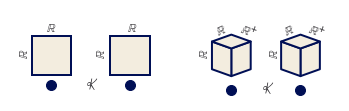
\includegraphics[width=\columnwidth]{fiber.png}
  \caption{These two datasets have the same base space \dbase. The plane is a representation of the fiber $\dfiber=\reals\times\reals$ for the variables (time, temperature) from \autoref{fig:intro:equivariance}, while the cube is the fiber $\reals\times\realsp\times\reals$ associated with (time, wind=(speed, direction))}
  \label{fig:math:data:fiber}
\end{figure}

In \autoref{fig:math:data:fiber} the plane fiber has components (\emph{time}, \texttt{datetime}, \reals) and (\emph{temperature}, \texttt{float}, \reals), while the cube fiber has components (\emph{time}, \texttt{datetime}, \reals) and (\emph{wind}, \texttt{wind}, \(\realsp\times\reals)\)) which encodes (\emph{speed}, \emph{direction}). 


\subsubsection{Equivariant Variable Properties: Monoid Actions}
\label{sec:math:data:monoid}
While structure on a set of values is often described algebraically as operations or through the actions of a group, for example Steven's measurement scales \cite{stevensTheoryScalesMeasurement1946, leaFormalizationMeasurementScale}, we generalize to monoids to support partial orderings. A partial ordering allows for multiple measurement values to have the same rank\cite{fongInvitationAppliedCategory2019}, which is useful for visualizing many types of multi indicator systems\cite{bruggemannRankingPrioritizationMultiindicator2011}. 

A monoid \cite{Monoid2021} $\monoid$ is a set with an associative binary operator $\ast:\monoid \times \monoid\rightarrow \monoid$. A monoid has an identity element $e\in \monoid$ such that $e\ast a= a \ast e = a$ for all $a \in \monoid$. As defined on a component of \dfiber, a left monoid action \cite{SemigroupAction2021,nlab:action} of $\monoid_i$ is a set $\dfiber_i$ with an action $\bullet: \monoid\times \dfiber_i \rightarrow \dfiber_i$ with the properties of associativity and identity. As with the fiber \dfiber\, the total monoid space \monoid\ is the cartesian product
\begin{equation}\label{eq:math:data:monoid:decompose}
\monoid= \monoid_{0} \times \ldots \times \monoid_{i}\times \ldots \times\ldots \monoid_{n}
\end{equation}
of each monoid $\monoid_{i}$ on $\dfiber_{i}$.  The monoid is also added to the specification of the fiber $(\fname_i,\, \ftype_i,\, \fttype\, \monoid_i)$

Defining the monoid actions on the components serves as the basis for identifying the invariance\cite{kindlmannAlgebraicProcessVisualization2014} that must be preserved in the visual representation of the component. Monoids are commonly found in functional programming because a property of monoids is that the components can be composed into complex transformation pipelines \cite{yorgeyMonoidsThemeVariations}. For example, a component that converts \(\dfiber_i=time\) with \(\monoid_i\) to hours can be combined with a component that shifts \(time\) by 2 hours to yield \(hours_2\) with the same \(monoid_i\). 


\subsubsection{Base Space: Continuity}
\label{sec:math:data:base}

 The base space \dbase\ acts as an indexing space, as emphasized by Butler\cite{butlerVectorBundleClassesForm1992,butlerVisualizationModelBased1989}, to express how the records in \dtotal\ are connected to each other. This is similar the notion of structural \textit{keys} with associated \textit{values} proposed by Munzner\cite{munznerVisualizationAnalysisDesign2014}, but our model treats keys as a pure reference to topology. Decoupling the keys from their semantics allows the metadata to be altered facilitates encoding of data where the independent variable may not be clear; for example the growth of a plant is dependent on both time and sunlight, and changing the changing the coordinate system or time resolution should have no effect on how the records are connected to each other. 
 
  \begin{figure}[htb]
    \centering % avoid the use of \begin{center}...\end{center} and use \centering instead (more compact)
    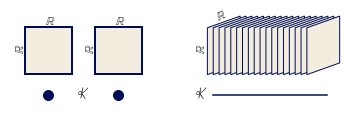
\includegraphics[width=\columnwidth]{base.png}
    \caption{These two datasets have the same fiber space $\dfiber=\reals\times\reals$. For example, the left dataset is a set of discrete (\textit{time}, \textit{temperature}) records while the right is a 1D continuous function over the interval $\left[0,1\right]$ with return values of the form (\textit{time}, \textit{temperature}).}
    \label{fig:math:data:base}
   \end{figure}
 As illustrated in ~\autoref{fig:math:data:base}, \dbase\ can have any number of dimensions, can be continuous or discrete, and is somewhat independent of the dimensions of the fiber. Every $\dbasepoint \in \dbase$ has a corresponding fiber $\dfiber_k$ because \dbase\ is the quotient space\cite{QuotientSpaceTopology2020,aurouxMath131Introduction} of \dtotal. As with \autoref{eq:math:data:fiber:decompose} and \autoref{eq:math:data:monoid:decompose}, we can decompose the total space into component bundles
 \begin{equation}\label{eq:math:data:base:decompose}
     \pi:\dtotal_1\oplus\ldots\oplus \dtotal_i \oplus\ldots \oplus \dtotal_n \rightarrow \dbase
 \end{equation}
 such that \(\monoid_{i}\) acts on component bundle \(\dtotal_i\). The \dbase\ remains the same because the connectivity of records does not change just because there are fewer components in each record. By encoding this continuity in the model as \dbase\, the data model now explicitly carries information about its structure such that the implicit assumptions of the visualization algorithms are now explicit. The explicit topology is a concise way of distinguishing visualizations that appear identical, for example heatmaps and images.  

 \subsubsection{Section: Values}
 \label{sec:math:data:section}
 


 \begin{figure}[htb]
  \centering % avoid the use of \begin{center}...\end{center} and use \centering instead (more compact)
  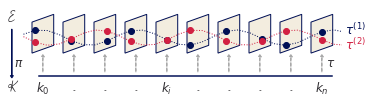
\includegraphics[width=\columnwidth]{fiberbundle.png}
  \caption{Each section in the fiber bundle is a unique continuous map from base space to fiber encoding a set of records in the dataset. For example, the two sections $\dsection^{(1)}$ and $\dsection^{(2)}$ each encode a timeseries from a different weather station.}
  \label{fig:math:data:section}
 \end{figure}

 While the projection function $\pi:\dtotal \rightarrow\dbase$ ties together the base space \dbase\ with the fiber \dfiber, a section $\dsection: \dbase\rightarrow \dtotal$ encodes a dataset. A section function takes as input location $\dbasepoint \in \dbase$ and returns a record $\delement \in \dtotal$. For any fiber bundle, there exists a map
 \begin{equation}
     \begin{tikzcd}
         \dfiber \arrow[r, hook] & \dtotal \arrow[d, "\pi"'] \\
                           & \dbase \arrow[u, "\dsection"', bend right]
     \end{tikzcd}
 \end{equation}
  such that $\pi(\dsection(\dbasepoint)) = \dbasepoint$. The set of all global sections is denoted as $\Gamma(\dtotal)$. As illustrated in \autoref{fig:math:data:section}, the section is a continuous mapping from a location $\dbasepoint \in \dbase$ on the base space to a record $\delement \in \dfiber$ in the fiber. Assuming a trivial fiber bundle $\dtotal = \dbase \times \dfiber$, a section
 \begin{equation}
     \label{eq:section_return}
     \dsection(\dbasepoint) = (\dbasepoint, (g_{\dfiber_{0}}(\dbasepoint), \ldots, g_{\dfiber_{n}}(\dbasepoint)))
 \end{equation}
 returns a record for each \dbasepoint. The index function $g: \dbase \rightarrow \dfiber$ into each fiber component returns a value in the component. This formulation of the section also holds on locally trivial sections of a non-trivial fiber bundle. As with \autoref{eq:math:data:fiber:decompose} and \autoref{eq:math:data:base:decompose}, \dsection\ can be decomposed into components 
 \begin{equation}
 \label{eq:math:data:section:decompose}
 \dsection= (\dsection_0,\ldots, \dsection_i, \dots, \dsection_n) 
 \end{equation}
 where each section $\dsection_i$ maps into a record on a component $\dfiber_i \in \dfiber$. This allows for accessing the data component wise in addition to accessing the data in terms of its location over \dbase.

 \subsubsection{Sheafs}
 \label{sec:math:data:sheaf}
A sheaf is a mathematical structure for defining collections of objects\cite{ghristElementaryAppliedTopology2014, ghristHomologicalAlgebraData2018,urbanikBriefIntroductionSchemes} on mathematical spaces. On the fiber bundle \dtotal, we can describe a sheaf as the collection of local sections $\iota^{*}\dsection$
 \begin{equation}
     \label{eq:sheaf}
     \begin{tikzcd}[column sep=huge]
         \iota^*\dtotal \arrow[d, "\pi"'] \arrow[r, "\iota^*", hook]             & \dtotal \arrow[d, "\pi"']                  \\
         U \arrow[r, "\iota", hook] \arrow[u, "\iota^{*}\dsection"', bend right] & \dbase \arrow[u, "\dsection"', bend right]
     \end{tikzcd}
 \end{equation}
which are sections of \dtotal\ pulled back over local neighborhood $U \subset \dtotal$ via the inclusion map \(\iota:\dtotal\rightarrow U\). The collation of sections enabled by sheafs is necessary for navigation techniques such as pan and zoom\cite{NekrasovskiEvaluationPanZoom2006} and dynamically updated visualizations such as sliding windows\cite{crouchDynamicGraphsSlidingwindow2013,chuTimeSeriesSegmentation1995}

 \subsection{Graphic Bundle}
 \label{sec:math:graphic}  
We introduce a graphic bundle to hold the essential information necessary to render a graphical design constructed by the artist. As with the data, we can represent the target graphic as a section \gsection\ of a bundle  $(\gtotal, \gbase, \pi, \gfiber)$
\begin{equation}
  \begin{tikzcd}[ampersand replacement=\&]
      \gfiber \arrow[r, hook] \& \gtotal \arrow[d, "\pi"'] \\
                        \& \gbase \arrow[u, "\gsection"', bend right]
  \end{tikzcd}
\end{equation}
where \gsection\ is a fully specified graphic such that it is an abstraction of rendering. To fully specify the visual characteristics of the image, we construct a fiber \gfiber\ that is an infinite resolution version of the target space. Typically \gtotal\ is trivial and therefore sections can be thought of as mappings into \gfiber. In this work, we assume a 2D opaque image $\gfiber=\reals^5$ with elements $(x,\, y,\, r,\, g,\, b) \in \gfiber$ such that a rendered graphic only consists of 2D position and color. By abstracting the target display space as \gfiber, the model can support different targets, such as a 2D screen or 3D printer. 

\subsubsection{Equivariant Topology: Graphic Base Space}
\label{sec:math:graphic:base}
\begin{figure}[htb]
  \centering % avoid the use of \begin{center}...\end{center} and use \centering instead (more compact)
  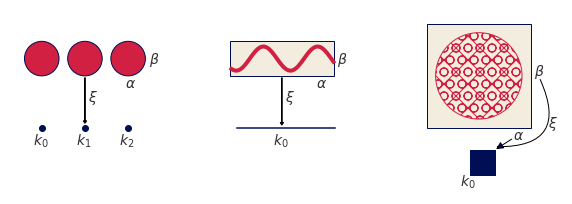
\includegraphics[width=\columnwidth]{retraction_maps.png}
  \caption{The 0D scatter \dbasepoint\ and 1D line \dbasepoint\ are thickened into \gbase\ with coordinates $\gbasepoint=(\gx, \gy)$ that are a region in an idealized 2D screen. The image has the same dimension in \gbase\ as in \dbase.}
  \label{fig:math:graphic:base}
 \end{figure}

Just as the \dbase\ encodes the connectivity of the records in the data, we propose an equivalent \gbase\ that encodes the connectivity of the rendered elements of the graphic. Formally, we require that \dbase\ be a deformation retract\cite{RetractionTopology2020} of \gbase\ so that \dbase\ and \gbase\ have the same homotopy. The surjective map $\vindex: \gbase \rightarrow \dbase$ 
\begin{equation}
    \begin{tikzcd}
        \dtotal \arrow[d, "\pi"'] & \gtotal \arrow[d, "\pi"'] \\
        \dbase                   & \gbase \arrow[l, "\vindex"']
    \end{tikzcd}
\end{equation}
goes from region $\gbasepoint \in \gbase_{\dbasepoint}$ to its associated point $\gbasepoint$. While \gbase\ must have the same continuity as \dbase\, it is sometimes the  thickened version shown in \autoref{fig:math:graphic:base}. This thickening is necessary when the dimensionality of \dbase\ is less than the dimensionality of the target display. For example, a \dbasepoint\ that is a point in 0D \dbase\ cannot be represented on screen unless it is thickened to 2D to encode the connectivity of the points in \gfiber\ that visually represent the record at \dbasepoint. The \vindex\ mapping is critical to interactive visualizations as it is the map from a region on screen to the data associated with that region. One example is to fill in details in a hover tooltip, another is to convert region selection on \gbase\ to a query on the data to access the corresponding record components on \dbase.

\subsection{Artist}
\label{sec:math:artist}
The topological artist \vartist\ is a map from the sheaf on a data bundle \dtotal\ which is $\mathcal{O}(\dtotal)$ to the sheaf on the graphic bundle \gtotal, $\mathcal{O}(\gtotal)$. 
\begin{equation}
    \vartist: \mathcal{O}(\dtotal) \rightarrow \mathcal{O}(\gtotal)
    \label{eq:math:artist:artist}
\end{equation}
that carries a homomorphism of monoid actions $\varphi: \monoid \rightarrow \monoid^{\prime}$ \cite{cegarraCohomologyMonoidsOperators2019}. Given \monoid\ on data $\mathscr{\dtotal}$ and $\monoid^{\prime}$ on graphic $\mathscr{\gtotal}$, we propose that artists $\mathscr{\vartist}$ are equivariant maps 
\begin{equation}
\vartist(m\cdot \delement) = \varphi(m)\cdot \vartist(\delement) 
\end{equation}
such that applying a monoid action $m \in \monoid$ to the data $\delement \in \mathscr{\dtotal}$ input to $\mathscr{\vartist}$ is equivalent to applying a monoid action $\varphi(\monoid) \in \monoid^{\prime}$ to the graphic $\vartist(\delement) \in \mathscr{\gtotal}$ output of the artist.

The monoid equivariant map has two stages: the encoders $\vchannel:\dtotal^{\prime} \rightarrow \vtotal$ convert the data components to visual components, and the assembly function $\vmark: \vtotalpull \rightarrow \gtotal$ composites the fiber components of \vtotalpull\ into a graphic in \gtotal.
\begin{equation}
    \label{eq:math:artist:diagram}
    \begin{tikzcd}
        \dtotal \arrow[r, "\vchannel"] \arrow[rd, "\pi"'] & \vtotal \arrow[d, "\pi"] & \vindex^*\vtotal \arrow[r, "\vmark"] \arrow[d, "\vindex^*\pi"'] \arrow[l, "\vindex^*"'] & \gtotal \arrow[ld, "\pi"] \\
                                              & \dbase                  & \gbase \arrow[l, "\vindex"']                                              &                    
        \end{tikzcd}
\end{equation}
\vtotalpull\ is the visual bundle \vtotal\ pulled back over \gbase\ via the equivariant continuity map $\vindex:\gbase \rightarrow \dbase$ introduced in \autoref{sec:math:graphic:base}. The visual bundle $(\vtotal,\,\dbase,\,\pi ,\,\vfiber)$ is the space of possible parameters of a visualization type, such as a scatter or line plot. As with the data and graphic bundles, the visual bundle is defined by the projection map $\pi$
\begin{equation}
    \begin{tikzcd}[ampersand replacement=\&]
        \vfiber \arrow[r, hook] \& \vtotal \arrow[d, "\pi"'] \\
                          \& \dbase \arrow[u, "\vsection"', bend right]
    \end{tikzcd}
\end{equation}
where \vsection\ is the visual variable encoding, as described by Bertin \cite{bertinSemiologyGraphicsDiagrams2011a}, of the data section \dsection. The visual fiber \vfiber\ is defined in terms of the input parameters of the visualization library's plotting functions; by making these parameters explicit components of the fiber, we can build consistent definitions and expectations of how these parameters behave. The functional decomposition of the visualization artist facilitates building reusable components at each stage of the transformation because the equivariance constraints are defined on \vchannel, \vmark, and \vindex. We name this map the artist as that is the analogous part of the  Matplotlib\cite{hunterArchitectureOpenSource} architecture that builds visual elements.

\subsubsection{Visual Component Maps}
\label{sec:math:artist:nu}
 We define the visual transformers \vchannel\ 
\begin{equation}
  \label{eq:math:artist:nu}
  \{\vchannel_{0}, \ldots, \vchannel_{n}\}: \{\dsection_{0}, \ldots, \dsection_{n}\} \mapsto \{\vsection_{0}, \ldots, \vsection_{n}\}
\end{equation}
as the set of equivariant maps $\vchannel_i: \dsection_i \mapsto \vsection_i$. Given $\monoid_i$ is the monoid action on $\dtotal_i$ and that there is a monoid ${\monoid_i}^{\prime}$ on $\vtotal_i$, then there is a monoid homomorphism from $\varphi:\monoid_i \rightarrow {\monoid_i}^{\prime}$ that \vchannel\ must preserve. As mentioned in \autoref{sec:math:data:monoid}, monoid actions define the structure on the fiber components and are therefore the basis for equivariance. A validly constructed \vchannel\ is one where the diagram of the monoid transform $m$ commutes
\begin{equation}
  \label{eq:math:artist:nu_commute}
\begin{tikzcd}
  \dtotal_i \arrow[r] \arrow[r, "\vchannel_i"] \arrow[d, "m_{\delement}"'] & \vtotal_i \arrow[d, "m_{\velement}"] \\
  \dtotal_i \arrow[r, "\vchannel_i"]                           & \vtotal_i               
\end{tikzcd}
\end{equation}
such that applying equivariant monoid actions to $\dtotal_{i}$ and $\vtotal_{i}$ preserves the map $\vchannel_{i}: \dtotal_{i}\rightarrow \vtotal_{i}$. In general, the data fiber $\dfiber_{i}$ cannot be assumed to be of the same type as the visual fiber $\vfiber_{i}$ and the actions of \monoid\ on $\dfiber_{i}$ cannot be assumed to be the same as the actions of $\monoid^{\prime}$ on \vfiber; therefore an equivariant $\vchannel_i$ must satisfy the constraint  
\begin{equation}
\vchannel_i(m_{\delement}(\dtotal_i)) = \varphi(m_{\delement})(\vchannel_i(\dtotal_i))
\label{eq:math:artist:nu:equivariance}
\end{equation} 
such that $\varphi$ maps a monoid action on data to a monoid action on visual elements. However, we can construct a monoid action of \monoid\ on $\vfiber_{i}$ that is compatible with a monoid action of \monoid\ on $\dfiber_{i}$. We can compose the monoid actions on the visual fiber $\monoid^{\prime} \times \vfiber_{i} \rightarrow \vfiber_{i}$ with the homomorphism $\varphi$ that takes \monoid\ to $\monoid^{\prime}$. This allows us to define a monoid action on \vfiber\ of \monoid\ that is $(m, \velement) \rightarrow \varphi(m)\bullet\velement$. Therefore, without a loss of generality, we can assume that an action of \monoid\ acts on $\dfiber_{i}$ and on $\vfiber_{i}$ compatibly such that $\varphi$ is the identity function. 

\begin{figure}[htb]
  \centering
  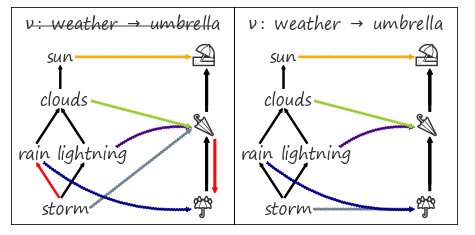
\includegraphics[width=1\columnwidth]{figures/partial_fixed.png}
  \caption{As highlighted by the red arrows, the equivariance constraint is not met because \(rain\geq storm\), but \(\vchannel(rain) \leq \vchannel(storm)\). Instead, mapping \textit{storm} to the same element as \textit{rain} yields an equivariant \vchannel\ such that \(\vchannel(rain) \geq \vchannel(storm)\).}
  \label{fig:math:artist:nu}
\end{figure}

\begin{table}[H]
  \renewcommand{\arraystretch}{2}
  \begin{tabulary}{\columnwidth}{|llL|}\hline
      \textbf{scale} & \textbf{group} & \textbf{constraint}\\ \hline
      nominal & permutation &  $\text{if } \delement_1 \neq \delement_2 \text{ then } \vchannel (\delement_1) \neq\vchannel(\delement_2)$\\
      ordinal &  monotonic & $\text{if } \delement_1 \leq \delement_2 \text{ then } \vchannel (\delement_1) \leq \vchannel(\delement_2)$\\
      interval &  translation &  $\vchannel (x + c) = \vchannel(x) + c$ \\
      ratio &  scaling &  $\vchannel(xc) = \vchannel(x)*c $\\ \hline
  \end{tabulary}
  \label{tab:math:artist:nu}
\end{table}
We can state the conditions on \vchannel\ such that they cover the Stevens measurement scales\cite{stevensTheoryScalesMeasurement1946}, as defined in \autoref{tab:math:artist:nu}. This is because Stevens’ defined the measurement scales in terms of their mathematical group structure and a group is a monoid with inverses\cite{remlingAlgebraMath5353}. An example of monoid action equivariance is the preservation of partial ordering illustrated in \autoref{fig:math:artist:nu}.


\subsubsection{Visualization Assembly}
\label{sec:math:artist:q}
\begin{figure}[htb]
  \centering
  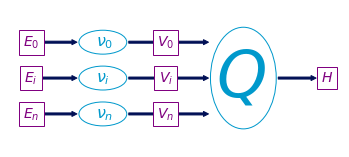
\includegraphics[width=\columnwidth]{path_of_q}
  \caption{The transform functions $\vchannel_i$ convert data $\dsection_i\in \dtotal$ to visual characteristics $\vsection_i \in \vtotal$, then \vmark\ assembles $\vsection_i$ into a graphic $\gsection \in \gtotal$.} 
  \label{fig:math:artist:q}
\end{figure}
As shown in \autoref{fig:math:artist:q}, \vchannel\ and \vmark\ are analogous to a  map-reduce operation: data components $\dtotal_{i}$ are mapped into visual components $\vtotal_{i}$ that are reduced into a graphic in \gtotal. The space of all graphics that \vmark\ can generate is the subset of graphics reachable via applying the reduction function $\vmark(\Gamma(\vtotal)) \in \Gamma(\gtotal)$ to the visual section $\vsection \in \Gamma(\vtotal)$. We formalize the expectation that visualization generation functions parameterized in the same way should generate the same functions as the equivariant map $\vmark: \vsection \mapsto \gsection$. We then define the constraint on \vmark\ such that if \vmark\ is applied to two visual sections $\vsection$ and $\vsection^{\prime}$ that generate the same \gsection\, then the output of $\vsection$ and $\vsection^{\prime}$ acted on by the same monoid $m$ must be the same.  We do not define monoid actions on all of $\Gamma(\gtotal)$ because there may be graphics $\gsection \in \Gamma(\gtotal)$ for which we cannot construct a valid mapping from \vtotal.
\begin{figure}[htb]
  \centering
  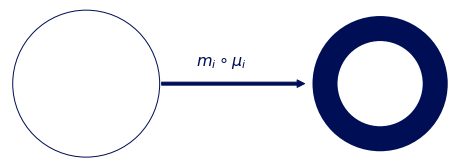
\includegraphics[width=\columnwidth]{diff_type_q.png}
  \caption{These two glyphs are generated by the same annulus \vmark\ function. The monoid action $m_i$ on edge thickness $\vsection_i$ of the first glyph yields the thicker edge ${\vsection_i}^{\prime}$ in the second glyph.}
  \label{fig:math:artist:graphic}
\end{figure}
Lets call the visual representations of the components $\Gamma(\vtotal)=X$ and the graphic $\vmark(\Gamma(\vtotal))=Y$
\begin{prop}
If for elements of the monoid $m \in \monoid$ and for all $\vsection, \vsection^{\prime} \in X$, we define the monoid action on $X$ so that it is by definition equivariant
\begin{equation}
\vmark(\vsection) = \vmark(\vsection^{\prime})\implies \vmark(m\circ\vsection) = \vmark(m\circ\vsection^{\prime})
\label{eq:math:artist:q}
\end{equation}
then a monoid action on $Y$ can be defined as $m\circ \gsection = \gsection^{\prime}$. If and only if \vmark\ satistfies \autoref{eq:math:artist:q}, we can state that the transformed graphic $\gsection^{\prime}=\vmark(m\circ \vsection)$ is equivariant to a monoid action applied on \vmark\ with input $\vsection \in \vmark^{-1}(\gsection)$ that must generate valid \gsection. 
\end{prop}

For example, given fiber $\vfiber=(xpos,\, ypos,\, color,\, thickness)$, then sections $\vsection=(0,0,0,1)$ and $\vmark(\vsection) = \gsection$ generates a piece of the thin hollow circle. The action $m=(e, e, e, x+2)$, where e is identity, translates \vsection\ to  $\vsection^{\prime}=(e,e,e,3)$ and the corresponding action on \gsection\ causes $\vmark(\vsection^{\prime})$ to be the thicker circle in \autoref{fig:math:artist:graphic}.

We formally describe a glyph as \vmark\ applied to the regions \dbasepoint\ that map back to a set of path connected components $\dbasepath \subset \dbase$ as input 
\begin{equation}
\dbasepath = \{\dbasepathpoint \in \dbase \text{ s. t. } \exists \gamma \text{ s.t. } \gamma(0)=\dbasepoint \text{ and }\gamma(1)=\dbasepathpoint\}
\end{equation}
where the path\cite{ConnectedSpace2020}  $\gamma$ from \dbasepoint\ to \dbasepathpoint\ is a continuous function from the interval [0,1]. We define the glyph as the graphic generated by $\vmark(\gbase_{\dbasepathpoint})$
\begin{equation}
  \begin{tikzcd}
      \gtotal \arrow[r, shift left] & \gbase_\dbasepathpoint \arrow[rr, "\vindex(\gbasepoint)", shift left] \arrow[l, "\gsection(\gbase_\dbasepathpoint)"] &  & \dbasepath_{\dbasepoint} \arrow[ll, "\vindex^{-1}(\dbasepath)"]
      \end{tikzcd}
  \label{eq:mark}
\end{equation}
such that for every glyph there is at least one corresponding region on \dbase, in keeping with the definition of glyph as any differentiable element put forth by Ziemkiewicz and Kosara\cite{ziemkiewiczEmbeddingInformationVisualization2009}. The primitive point, line, and area marks\cite{bertinSemiologyGraphicsDiagrams2011a,carpendaleVisualRepresentationSemiology} are specially cased glyphs.

\begin{figure}
  \centering
  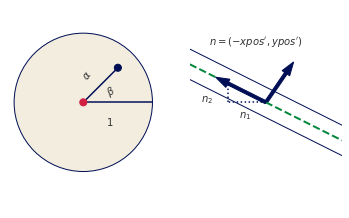
\includegraphics[width=\columnwidth]{base_q}
  \caption{The coordinates \(\gbasepoint=(\gx, \gy)\) dictate the color of the region in prerender space \gbase. When \vmark\ is applied over the whole disk \(\gbase_{\dbasepoint}\), it generates the graphical point mark. The line fiber is thickened with the derivative because the tangent the line needs to be pushed perpendicular to the tangent of (xpos, ypos) in order to have visible thickness.}
  \label{fig:math:artist:base}
\end{figure}

In \autoref{fig:teaser}, we illustrate the output of a minimal Q that will generate distinguishable graphical marks: non-overlapping scatter points, a non-infinitely thin line, and an image. The scatter plot can be defined as 
\begin{equation}
\vmark(xpos, ypos)(\alpha, \beta)
\label{eq:math:artist:q:scatter}
\end{equation}
with a constant \textit{size} and color $\gsection_{RGB} = (0,0,0)$ that are defined as part of \vmark. The position of this swatch of color can be computed relative to the location on the disc \((\alpha, \beta) \in \gbase_{\dbasepoint}\) as shown in \autoref{fig:math:artist:base}
\begin{align*}
x &= size *\alpha \cos(\beta) + xpos \\
y &= size *\alpha \sin(\beta) + ypos
\end{align*}
such that $\gsection(\gbasepoint) = (x, y, 0, 0, 0)$ colors the point (x,y) black. 
In contrast, the line plot 
\begin{equation}
\vmark(xpos, \hat{n}_{1}, ypos, \hat{n}_{2})(\alpha, \beta)
\label{eq:math:artist:q:line}
\end{equation}
in \autoref{fig:teaser} has a \vindex\ function that is not only parameterized on \dbasepoint\ but also on the $\alpha$ distance along \dbasepoint\ and corresponding region in \gbase. As shown in \autoref{fig:math:artist:base}, line needs to know the tangent of the data to draw an envelope above and below each (xpos,ypos) such that the line appears to have a thickness; therefore the artist takes as input the jet bundle \cite{JetBundle2020,musilovaCalculusVariationsJet2016} $\mathcal{J}^{2}(\dtotal)$ which is the data \dtotal\ and the first and second derivatives of \dtotal. The magnitude of the slope is $\lvert n \rvert = \sqrt{{n_{1}}^2 + {n_{2}}^2}$
such that the normal is  $\hat{n}_{1} = \frac{n_1}{\lvert n \rvert}, \; \hat{n}_{2} = \frac{n_2}{\lvert n \rvert}$ which yields components of \gsection\
\begin{align*}
 x = xpos(\vindex(\alpha)) &+ width*\beta\hat{n}_1(\vindex(\alpha)) \\
 y = ypos(\vindex(\alpha)) &+ width*\beta\hat{n}_2(\vindex(\alpha)) 
\end{align*}
where (x,y) look up the position $\vindex(\alpha)$ on the data and the derivatives $\hat{n}_1, \hat{n}_2$ . The derivatives are then multiplied by a $width$ parameter to specify the thickness.
In \autoref{fig:teaser}, the image 
\begin{equation}
\vmark(xpos, ypos, color)
\label{eq:math:artist:q:image}
\end{equation}
 is a direct lookup into  $\vindex:\gbase\rightarrow\dbase$. The indexing variables $(\alpha, \beta)$ define the distance along the space, which is then used by \vindex\ to map into \dbase\ to lookup the color values 
\begin{equation*}
R = R(\vindex(\alpha, \beta)), \; G = G(\vindex(\alpha, \beta)), \; B = B(\vindex(\alpha, \beta))
\end{equation*}
In the case of an image, the indexing mapper \vindex\ may do some translating to a convention expected by \vmark, for example reorientng the array such that the first row in the data is at the bottom of the graphic. 

\subsubsection{Assembly Factory}
\label{sec:math:artist:qhat}
The graphic base space \gbase\ is not accessible in many architectures, including Matplotlib; instead we can construct a factory function \vmarkd\ over \dbase\ that can build a \vmark. As shown in \autoref{eq:math:artist:diagram}, \vmark\ is a bundle map $\vmark: \vtotalpull\rightarrow \gtotal$ where \vtotalpull\ and \gtotal\ are both bundles over \gbase.
\begin{figure}[htb]
  \centering
    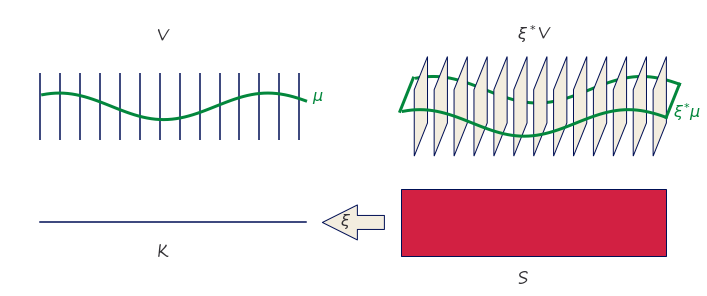
\includegraphics[width=1\columnwidth]{q_hat.png}
    \caption{Because the pullback of the visual bundle \vtotalpull\ is the replication of a \vsection\ over all points \gbasepoint\ that map back to a single \dbasepoint, we can constract a \vmarkd\ on \vsection\ over \dbasepoint\ that will fabricate the \vmark\ for the equivalent region of \gbasepoint\ associated to that \dbasepoint}
    \label{fig:math:artist:qhat}
\end{figure}

The preimage of the continuity map $\vpreimg \subset \gbase$ is such that many graphic continuity points $\gbasepoint \in \gbase_{\dbase}$ go to one data continuity point \dbasepoint; therefore, by definition the pull back of \vsection\
\begin{equation}
    \vtotalpull \mid_{\vpreimg} = \vpreimg \times \vfiber
\end{equation}
copies the visual fiber \vfiber\ over the the points \gbasepoint\ in graphic space \gbase\ that correspond to one \dbasepoint\ in data space \dbase. This set of points \gbasepoint\ are the preimage \vpreimg\ of \dbasepoint. 

As shown in \autoref{fig:math:artist:qhat}, given the section \vsectionpull\ pulled back from \vsection\ and the point $\gbasepoint \in \vpreimg$, there is a direct map $(\dbasepoint, \vsection(\dbasepoint)) \mapsto (\gbasepoint, \vsectionpull(\gbasepoint))$  from \vsection\ over \dbasepoint\ to the section \vsectionpull\ over \gbasepoint. This means that the pulled back section $\vsectionpull(\gbasepoint) = \vindex^*(\vsection(\dbasepoint))$ is the section \vsection\ copied over all \gbasepoint such that \vsectionpull\ is identical for all \gbasepoint\ where $\vindex(\gbasepoint) = \dbasepoint$. In \autoref{fig:math:artist:qhat} each dot on \vfiber\ is equivalent to the line on \vfiberpull. 

Given the equivalence between \vsection\ and \vsectionpull\ defined above, the reliance on \gbase\ can be factored out. When \vmark\ maps visual sections into graphics $\vmark: \Gamma(\vtotalpull) \rightarrow \Gamma(\gtotal)$, if we restrict \vmark\ input to \vsectionpull\ then the graphic section \gsection\ evaluated on a visual region \gbasepoint\
\begin{equation}
    \gsection(\gbasepoint) \coloneqq \vmark(\vsectionpull)(s)
    \label{eq:math:artist:qhat}
\end{equation}
 is defined as the assembly function \vmark\ with input \vsectionpull\ evaluated on \gbasepoint. Since the pulled back section \vsectionpull\ is the section \vsection\ copied over every graphic region $\gbasepoint \in \vpreimg$, we can define a \vmark\ factory function 
\begin{equation}
\label{eq:math:artist:qhat_q_s}
\vmarkd(\vsection(\dbasepoint))(\gbasepoint) \coloneqq \vmark((\vsectionpull)(\gbasepoint))
\end{equation} 
where \vmarkd\ with input \vsection\ is defined to \vmark\ that takes as input the copied section \vsectionpull\ such that both functions are evaluated over the same location $\vpreimg = \gbasepoint$ in the base space \gbase. Factoring out \gbasepoint\ from \autoref{eq:math:artist:qhat_q_s} yields
\begin{equation}
\vmarkd(\vsection(k)) = \vmark(\vsectionpull)
\label{eq:math:artist:qhat_k}
\end{equation}
where \vmark\ is no longer bound to input but \vmarkd\ is still defined in terms of \dbase. In fact, \vmarkd\ is a map from visual space to graphic space $\vmarkd:\Gamma(\vtotal) \rightarrow \Gamma(\gtotal)$ locally over \dbasepoint\ such that it can be evaluated on a single visual record  $\vmarkd:\Gamma(\vtotal_{\dbasepoint}) \rightarrow \Gamma(\gtotal\mid_{\vpreimg})$. This allows us to construct a \vmarkd\ that only depends on \dbase, such that for each $\vsection(\dbasepoint)$ there is part of $\gsection\mid_{\vpreimg}$. The construction of \vmarkd\ allows us to retain the functional map reduce benefits of \vmark\ without having to majorly restructure the existing pipeline for libraries that delegate the construction of \gsection\ to a back end such as Matplotlib.

\subsubsection{Composite and Reusable Artists}
Given the family of artists $(\dtotal_i: i\in I)$ on the same image, the + operator 
\begin{equation}
+ \coloneqq \underset{i\in I}{\sqcup} \dtotal_{i}
\end{equation}
defines a simple composition of artists. When artists share a base space $\dbase_2 \hookrightarrow \dbase_1$, a composition operator can be defined such that the artists are acting on different components of the same section. This type of composition is important for visualizations where elements update together in a consistent way, such as multiple views \cite{alboRadarComparativeEvaluation2016a, hullmanKeeping2018} and brush-linked views\cite{beckerBrushingScatterplots1987,bujaInteractiveData1991}. It is impractical to implement an artist for every single graphic; instead we implement an approximation of the equivalence class of artists 
\begin{equation}
\{\vartist \in \vartist^{\prime}: \vartist_{1} \equiv \vartist_{2}\}
\label{eq:math:artist:aprime}
\end{equation}
Roughly, two artists are equivalent if they have the same visual fiber \vfiber\, assembly function \vmark\, and continuity map \vindex. 

\section{Prototype}
\label{sec:code}
To build a prototype, we make use of the Matplotlib figure and axes artists \cite{hunterArchitectureOpenSource,hunterMatplotlib2DGraphics2007} so that we can initially focus on the data to graphic transformations and exploit the Matplotlib transform stack to transform data coordinates into screen coordinates. While the artist is specified in a fully functional manner in \autoref{eq:math:artist:diagram}, we implement our prototype in a heavily object oriented manner. We do so mostly to more easily manage function inputs, especially parameters that are passed through to the structurally functional transform and draw methods. 

\begin{minted}{python}
  fig, ax = plt.subplots()
  artist = Artist(E, V)
  ax.add_artist(artist)
\end{minted}
Building on the current Matplotlib artists which construct an internal representation of the graphic, \mintinline{python}{ArtistClass} acts as an equivalence class artist \vartisteq\ as described in \autoref{eq:math:artist:aprime}. The visual bundle \vtotal\ is specified as the \mintinline{python}{V} dictionary of the form \mintinline{python}|{parameter:(variable name, encoder)}| where parameter is a component in \vfiber, variable is a component in \dfiber, and the \vchannel\ encoders are passed in as functions or callable objects. The data bundle \dtotal\ is passed in as a \mintinline{python}{E} object. By binding data and transforms to \vartisteq\ inside \mintinline{python}{__init__}, the \mintinline{python}{draw} method is a fully specified artist \vartist\ as defined in \autoref{eq:math:artist:artist}.
\begin{minted}{python}
  class ArtistClass(matplotlib.artist.Artist): #A'
      def __init__(self, E, V, *args, **kwargs):
          # properties that are specific to the graphic
          self.E = E
          self.V = V 
          super().__init__(*args, **kwargs)
  
      def hat_Q(self, **args): 
          # set the properties of the graphic
  
      def draw(self, renderer):
          # returns K, indexed on fiber then key 
          tau = self.E.view(self.axes) 
          # visual channel encoding applied fiberwise 
          mu = {p: nu(tau(c))
                   for p, (c, nu) in self.V.items()} 
          self.hat_q(**mu)
          # pass configurations off to the renderer
          super().draw(renderer)
  \end{minted}
 The data is fetched in section \dsection\ via a \mintinline{python}{view} method on the data because the input to the artist is a section on \dtotal. The \mintinline{python}{view} method takes the \mintinline{python}{axes} attribute because it provides the region in graphic coordinates \gbase\ that can be used to query back into data to select a subset as described in \autoref{sec:math:data:sheaf}. To ensure the integrity of the section, \mintinline{python}{view} must be atomic, which means that the values cannot change after the method is called in draw until a new call in draw. We put this constraint on the return of the \mintinline{python}{view} method so that we do not risk race conditions. 
 
 The \vchannel\ functions are then applied to the data, as describe in \autoref{eq:math:artist:nu}, to generate the visual section \vsection that here is the object \mintinline{python}{V}. The conversion from data to visual space is simplified here to directly show that it is the encoding \vchannel\ applied to the component. The \mintinline{python}{q_hat} function that is \vmarkd,  as defined in \autoref{eq:math:artist:qhat_k}, is responsible for generating a representation such that it could be serialized to recreate a static version of the graphic. This artist is not optimized because we prioritized demonstrating the separability of \vchannel\ and \vmarkd. The last step in the artist function is handing itself off to the renderer. The extra \mintinline{python}{*arg, **kwargs} arguments in \mintinline{python}{__init__,draw} are artifacts of how these objects are currently implemented.

 \subsection{Scatter and Line Artists}
 \begin{figure}[H]
    \centering 
    \subfloat[\label{fig:code:scatter}]{%
      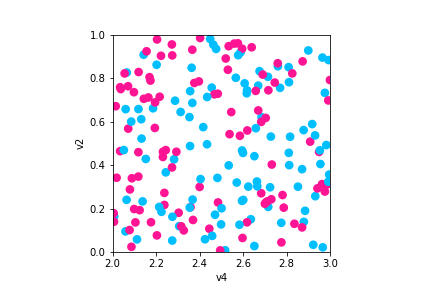
\includegraphics[width=0.5\columnwidth]{scatter_0.png}}
    \subfloat[\label{fig:code:line}]{%
      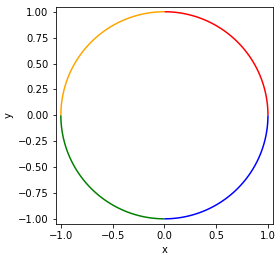
\includegraphics[width=0.5\columnwidth]{line_1.png}}
  \caption{Scatter plot and line plot implemented using prototype artists and data models, building on Matplotlib rendering.}
  \label{fig:code_scatter_line}
\end{figure}
The figure in \autoref{fig:code:scatter} is described by \autoref{eq:math:artist:q:scatter}. This is implemented via a \mintinline{python}{Line} object where the scatter marker shape is fixed as a circle, and the visual fiber components are x and y position and the facecolor and size of the marker. We only show the \mintinline{python}{q_hat} function here because the \mintinline{python}{__init__, draw} are identical the prototype artist. 

The \mintinline{python}{view} method repackages the data as a fiber component indexed table of vertices. Even though the \mintinline{python}{view} is fiber indexed, each vertex at an index \dbasepoint has corresponding values in section $\dsection(\dbasepoint_{i})$. This means that all the data on one vertex maps to one glyph.
\begin{minted}{python}
class Point(mcollections.Collection):
  def q_hat(self, x, y, s, facecolors): #\hat{Q}
    # construct geometries of circle glyphs
    self._paths = [mpath.Path.circle((xi,yi), radius=si) 
                for (xi, yi, si) in zip(x, y, s)] 
    # set attributes of glyphs, these are vectorized 
    # circles and facecolors are lists of the same size
    self.set_facecolors(facecolors)
\end{minted} 
In \mintinline{python}{q_hat}, the \vsection\ components are used to construct the vector path of each circular marker with center \texttt{(x,y)} and size \texttt{x} and set the colors of each circle. This is done via the \mintinline{python}{Path.circle} object. 
\begin{minted}{python}
class Line(mcollections.LineCollection):
  def q_hat(self, x, y, color): #\hat{Q}
    #assemble line marks as set of segments 
    segments = [np.vstack((vx, vy)).T for vx, vy 
                in zip(x, y)]
    self.set_segments(segments)
    self.set_color(color)
\end{minted}
To generate \autoref{fig:code:line}, the \mintinline{python}{Line} artist \mintinline{python}{view} method returns a table of edges. Each edge consists of (x,y) points sampled along the line defined by the edge and information such as the color of the edge. As with \mintinline{python}{Point}, the data is then converted into visual variables. In \mintinline{python}{q_hat}, described by \autoref{eq:math:artist:q:line}, this visual representation is composed into a set of line segments, where each segment is the array generated by \mintinline{python}{np.vstack((vx, vy))}. Then the colors of each line segment are set. The colors are guaranteed to correspond to the correct segment because of the atomicity constraint on view. 

\subsubsection{Visual Encoders}
The visual parameter serves as the dictionary key because the visual representation is constructed from the encoding applied to the data  $\vsection = \vchannel \circ \dsection$. For the scatter plot, the mappings for the visual fiber components $\vfiber=(x,y, facecolors, s)$ are defined as
\begin{minted}{python}
cmap =  color.Categorical({'true':'deeppink', 
                           'false':'deepskyblue'}) 
# {P_i name:{'name':c_i, 'encoder:\nu_i}}
V = {'x': {'name': 'v4', 'encoder': lambda x: x}, 
     'y': {'name': 'v2', 'encoder': lambda x: x},
     'facecolors': {'name':'v3', 'encoder': cmap}, 
     's':{'name': None , 
          'encoder': lambda _: itertools.repeat(.02)}}
\end{minted}
where \mintinline{python}{lambda x: x} is an identity \vchannel, \mintinline{python}|{'name':None}| maps into \vfiber\ without corresponding \dsection\ to set a constant visual value, and \mintinline{python}{color.Categorical} is a custom \vchannel\ implemented as a class for reusability.  A test for equivariance, as described in \autoref{eq:math:artist:nu:equivariance}, can be implemented trivially
\begin{minted}{python}
#\nu_i(m_r(E_i)) = \varphi(m_r)(\nu_i((E_i))
def test_nominal(values, encoder):
    m1 = list(zip(values, encoder(values)))
    random.shuffle(values)
    m2 = list(zip(values, encoder(values)))
    assert sorted(m1) == sorted(m2)
\end{minted}
but is currently factored out of the artist for clarity. 

\subsubsection{Data Model}
The data input into the \mintinline{python}{Artist} will often be a wrapper class around an existing data structure. This wrapper object must specify the fiber components \dfiber\ and connectivity \dbase\ and have a \mintinline{python}{view} method that returns an atomic object that encapsulates \dsection. To support specifying the fiber bundle, we define a \mintinline{python}{FiberBundle} data class\cite{DataclassesDataClasses}

\begin{minted}{python}
@dataclass
class FiberBundle:
    K: dict #{'tables': []}
    F: dict #  {variable name: type}
\end{minted}
that asks the user to specify the the properties of \dfiber\ and the \dbase\ connectivity as either discrete vertices or continuous data along edges. To generate the scatter plot and the line plot, the distinction is in the \mintinline{python}{tau} method that is the section. 
\begin{minted}{python}
class PointData:     
    def __init__(self):
      FB = FiberBundle({'tables': ['vertex']},  
                       {'v1': float, 'v2': str, 'v3': float})
    def tau(self, k):
      return # tau evaluated at one point k

class LineData:
  def __init__(self):
    FB = FiberBundle({'tables': ['edge']},  
                     {'x': float, 'y': float, 'color': str})
  def tau(self, k):
    return # tau evaluated on interval k
\end{minted}
The discrete \mintinline{python}{tau} method returns a record of discrete points, akin to a row in a table, while the line\mintinline{python}{tau} returns a sampling of points along an edge \dbasepoint.
\begin{minted}{python}
  def view(self, axes):
      table = defaultdict(list)
      for k in self.keys:
          table['index'].append(k)
          for (name, value) in zip(self.FB.fiber.keys(), 
                                   self.tau(k)[1]):
              table[name].append(value)
      return table
\end{minted}
In both cases, the \mintinline{python}{view} method packages the data into a data structure that the artist can unpack via data component name, akin to a table with column names when \dbase\ is 0 or 1 D. 

\begin{figure}[htb]
  \centering 
  \subfloat[\label{fig:code:line:arc}]{%
    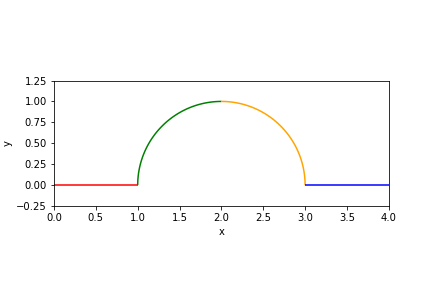
\includegraphics[width=0.5\columnwidth]{linec_1.png}}
  \subfloat[\label{fig:code:line:step}]{%
    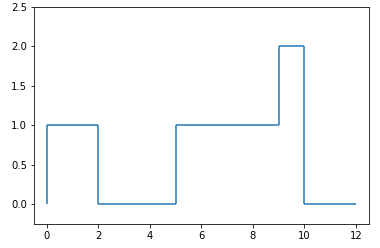
\includegraphics[width=0.5\columnwidth]{lined_1.png}}
\caption{Continuous and discontinuous lines as defined via the same data model, and generated with the same \vartisteq \mintinline{python}{Line}}
\label{fig:code:multilines}
\end{figure}
The graphics in figure \autoref{fig:code:multilines} are made using the \mintinline{python}{Line} artist and the \mintinline{python}{GraphData} data source where if told that the data is connected, the data source will check for that connectivity by constructing an adjacency matrix. The multicolored line is a connected graph of edges with each edge function evaluated on 1000 samples, 
\begin{minted}{python}
GraphData(FB, edges, verticies, num_samples=1000, connect=True)
\end{minted}
while the stair chart is discontinuous and only needs to be evaluated at the edges of the interval 
\begin{minted}{python}
GraphData(FB, edges, verticies, num_samples=2, connect=False)
\end{minted}
such that one advantage of this model is it helps differentiate graphics that have different artists from graphics that have the same artist but make different assumptions about the source data. 

\section{Discussion}
This work contributes a functional model of the structure-preserving maps from data to visual representation to guide the development of visualization libraries, thereby providing a means to express the constraints of preserving the data continuity in the graphic and faithfully translating the properties of the data variables into visual variables. Combining Butler's proposal of a fiber bundle model of visualization data with Spivak's formalism of schema lets this model support a variety of datasets, including  discrete relational tables, multivariate high resolution spatio temporal datasets, and complex networks. Decomposing the artist into encoding \vchannel, assembly \vmark, and reindexing \vindex\ provides the specifications that the graphic must have continuity equivalent to the data, and that the visual characteristics of the graphics are equivariant to their corresponding components under monoid actions. This model defines these constraints on the transformation function such that they are not specific to any one type of encoding or visual characteristic. Encoding the graphic space as a fiber bundle provides a structure rich abstraction of the target graphical design in the target display space. The toy prototype built using this model validates that is usable for a general purpose visualization tool since it can be iteratively integrated into the existing architecture rather than starting from scratch. Factoring out graphic formation into assembly functions allows for much more clarity in how they differ. This prototype demonstrates that this framework can generate the fundemental point (scatter plot) and line (line chart) marks. 

\subsection{Limitations}
Our model and prototype are deeply tied to Matplotlib's existing architecture, so it has not yet been worked through how the model generalizes to libraries such as VTK or D3. Even though the model is designed to be backend and format independent, it has only been tested against PNGs rendered with AGG\cite{shemanarevAntiGrainGeometry}. It is unknown how this framework interfaces with high performance rendering libraries such as openGL\cite{CarsonOpenGL1997} that implement different models of \gsection. While our model supports equivariance of figurative glyphs \cite{byrneAcquiredCodesMeaning2016} generated from data components\cite{beckfeathers2014,byrneFigurativeFramesCritical2017}, it cannot evaluate the semantic accuracy of the figurative representation. Effectiveness criteria\cite{mackinlayAutomaticDesignGraphical1987,chambersGraphicalMethodsData1983a} are out of scope.

\subsection{Future Work}
More work is needed to formalize the composition operators and equivalence class \vartisteq and  we need to implement artists that demonstrate that the model can underpin a minimally viable library, foremost an image\cite{haber1990visualization,hansen2011visualization}, a heatmap\cite{wilkinsonHistoryClusterHeat2009,loua1873atlas}, and an inherently computational artist such as a boxplot\cite{wickham40YearsBoxplots2011}. Since this model formalizes notions of structure preservation, it can serve as a good base for tools that assess quality metrics\cite{bertiniQualityMetricsHighdimensional2011a} or invariance \cite{kindlmannAlgebraicProcessVisualization2014}. While this paper formulates visualization in terms of monoidal action homomorphisms between fiber bundles, the model lends itself to a categorical formulation\cite{fongInvitationAppliedCategory2019,milewskiCategoryTheoryProgrammers} that could be further explored. 

\section{Conclusion}
The data model and functional transform refactor presented here allows bulding block libraries to better support domain specific libraries without having to explicitly take in the specific data structure and visualization needs of those domains. Adopting this model would induce a separation of data representation and visual representation that, for example, in Matplotlib is so entangled that it has lead to a brittle and sometimes incoherent API and internal code base. A refactor driven by TEAM would result in components that can be be guaranteed to preserve continuity and structure, as defined by the domain specific library developers, without having to fold domain specific assumptions back into the base library. 

%% if specified like this the section will be committed in review mode
\acknowledgments{
The authors wish to thank the Matplotlib development team for their invaluable feedback along the way, particulary Bruno Beltran, Eric Schles and Chana Tilevitz for idenfiying the confusing bits, Nicolas Kruchten for articulating the framing and Marc Hanwell, Lev Manovich, Robert Haralick and Huy Vo for invaluable feedback on various iterations. This paper is indebted to Kindlmann and Scheidegger's \cite{kindlmannAlgebraicProcessVisualization2014} for serving as a model and Munzner's guide to writing visualization papers. This project has been made possible in part by grant number 2019-207333 from the Chan Zuckerberg Initiative DAF, an advised fund of Silicon Valley Community Foundation.}

%\bibliographystyle{abbrv}
\bibliographystyle{abbrv-doi}
%\bibliographystyle{abbrv-doi-narrow}
%\bibliographystyle{abbrv-doi-hyperref}
%\bibliographystyle{abbrv-doi-hyperref-narrow}
\bibliography{../draft/glasslab_viz.bib}

\end{document}

